\begin{frame}
	\frametitle{Învătarea din observații - Amintire}
	
	\begin{block}{Problema Estimării (Antrenării) Modelului}
		\justifying		
		Dându-se un set de secvențe observate \alert{$\mathcal{O} = [O_1 O_2 \cdots O_L]$}, 
		cum ajustam \alert{parameterii} \alert{$\lambda=(A,B,\Pi)$} 
		ai unui MMA care incearcă să explice cel mai bine acele observații?
  	\end{block}	
  	\pause
	\vspace*{1em}
  	
  	\begin{block}{}
  		\justifying
		Secvențele de observații folosite pentru ajustarea parametrilor modelului se numesc secvențe 
		\alert{de antrenare}.\\
		Problema antrenării este esențiala - ea permite crearea celor mai bune modele pentru fenomene reale.
  	\end{block}
\end{frame}


\begin{frame}
	\frametitle{Învătarea din observații - Abordare}
	\pause
		
	\begin{block}{\alert{Problemă}}
		\justifying		
		Nu se cunoaște o metodă analitică de cautare a parametrilor modelului care \emph{maximizeaza} probabilitatea
		secvențelor observate.
  	\end{block}
	\vspace*{1em}
  	\pause
  	
  	\begin{block}{Soluție}
		\justifying
  		Putem totuși găsi $\lambda = (A, B, \Pi)$, astfel încât $\max_{\lambda} P(O \vert \lambda)$ corespunde
  		unui \alert{maxim local}, utilizând o \alert{procedură iterativă} precum \emph{algoritmul Baum-Welch}.\\
  		Această metodă este o instanță a \emph{algoritmului EM (Expectation Maximization) \citep{dempster1977maximum}} 
  		pentru cazul MMA.
  	\end{block}
  	
\end{frame}

\begin{frame}[fragile, t]
	\frametitle{Algoritmul Baum-Welch (I)}
	Procedura în descriere conceptuală:	
	\vspace*{0.25em}
	\footnotesize{
	\begin{enumerate}
		\item Avem MMA $\lambda = (A, B, \Pi)$ și o secvență observată $O$%
		\vspace*{0.25em}
		\pause
		
		\item Calculăm folosindu-ne de parametrii $\alpha_t(i)$ și $\beta_t(i)$			
			\begin{itemize}
				\item	$\scriptstyle 	\mbox{\scriptsize{nr. estimat de tranziții din }} S_i 
										\mbox{\scriptsize{, pentru fiecare} } 
				1 \le i \le N$%
				\vspace*{0.5em}
				\item	$\scriptstyle 	\mbox{\scriptsize{nr. estimat de tranziții din }} S_i 
										\mbox{ \scriptsize{la }} S_j 
										\mbox{\scriptsize{, pentru fiecare }} 1 \le i \le N, 1 \le j \le N$%
				\vspace*{0.5em}
				\item 	$\scriptstyle	\mbox{\scriptsize{nr. estimat de vizite în }} S_j 
										\mbox{\scriptsize{ observând simbolul }} v_k
										\mbox{\scriptsize{, pentru fiecare }} 1 \le j \le N, 1 \le k \le M$%
			\end{itemize}
		\vspace*{0.25em}		
		\pause
		
		\item Daca modelul este corect ne așteptăm ca
			\begin{enumerate}
				\item[(a)] $\scriptstyle \Pi_i = \mbox{{\scriptsize nr. estimat de vizite în starea }} 
													S_i \mbox{\small{ la momentul }} (t=1) = \bar{\Pi_i} $%
				\vspace*{0.5em}
				\item[(b)] $\scriptstyle a_{i,j} = \frac{\mbox{\scriptsize{nr. estimat de tranziții din }} S_i 
											\mbox{\scriptsize{ la }} S_j}
											{\mbox{\scriptsize{nr. estimat de tranziții din }} S_i} = \bar{a_{i,j}}$%
				\vspace*{0.5em}
				\item[(c)] $\scriptstyle b_{j,k} = \frac{\mbox{\scriptsize{nr. estimat de vizite în }} S_j 
											\mbox{\scriptsize{ observând simbolul }} v_k}
											{\mbox{\scriptsize{nr. estimat de vizite în }} S_j} = \bar{b_{j,k}}$%
			\end{enumerate}
		\vspace*{0.25em}		
		\pause
		
		\item Vedem că raporturile calculate din presupunerea noastră explică mai bine observația decât parametrii
				anteriori, i.e. $P(O \vert \bar{\lambda}) > P(O \vert \lambda) $%
		\vspace*{0.25em}
		\pause
		\item Atunci repetăm procesul până ce suntem mulțumiți (convergență: 
				$P(O \vert \bar{\lambda}) - P(O \vert \lambda) \le \epsilon$)
	\end{enumerate}
	}
\end{frame}

\begin{frame}[t]
	\frametitle{Algoritmul Baum-Welch (II)}
	\pause
	Definim întâi niște variabile auxiliare:
	
	\begin{block}{}    
    	$\xi_{t,i,j} = \xi_t(i,j) = P(q_t=s_i,q_{t+1}=s_j \vert O, \lambda)$\\
    	Probabilitatea de a fi în starea $s_i$ la momentul $t$ \textbf{și} în starea $s_j$ la momentul $t+1$,
    	condiționat de parametrii modelului curent și secvența observată.
	\end{block}
	\pause
	
	\begin{block}{}    
    	$ \gamma_{t,i} = \gamma_t(i) = P(q_t = s_i \vert O, \lambda)$\\
    	Probabilitatea de a fi în starea $s_i$ la momentul $t$, condiționat de parametrii modelului curent și 
    	secvența observată.
	\end{block}
	\vspace*{1em}
	\pause
	
	Din definiții rezultă că:\\
	$ \gamma_t(i) = \displaystyle\sum_{j=1}^{N}\xi_t(i,j)$
  	
\end{frame}

\begin{frame}[t]
	\frametitle{Algoritmul Baum-Welch (III)}
	\begin{columns}[T]
	
	\column{0.42\textwidth}
	\begin{figure}
  		\centering
		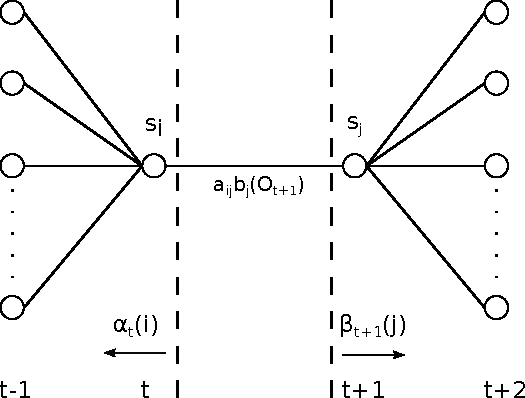
\includegraphics[height=0.40\textheight]{graphics/baum-welch/baum-welch-alg.pdf}
		\caption{
		\tiny{Secvența de operații necesară pentru calculul evenimentului mixt ca sistemul se află în
		starea $S_i$ la momentul $t$ și în starea $S_j$ la momentul $t+1$}
		} 
		\label{fig:baum-welch-alg}
  	\end{figure}	
	
	\column{0.58\textwidth}
		\begin{equation}		
		\alpha_{t,i}=P(o_1,o_2,\ldots,o_t, q_t = S_i \vert \lambda)
		\end{equation}
		
		\begin{equation}
		\beta_{t,i}=P(o_{t+1} o_{t+2} \cdots o_{T} \vert q_t = S_i, \lambda)
		\end{equation}
		\footnotesize
		
		\begin{equation}
			\begin{split}
		      \xi_t(i,j) & = \frac{\alpha_{t,i}\cdot a_{i,j} \cdot
		        b_j(o_{t+1}) \cdot \beta_{t+1,j}}
		      {P(O \vert \lambda)} \\
		      & = \frac{\alpha_{t,i}\cdot a_{i,j} \cdot b_j(o_{t+1}) \cdot
		        \beta_{t+1,j}}{
		        \displaystyle\sum_{k=1}^{N}\displaystyle\sum_{l=1}^{N}
		        \alpha_{t,k}\cdot a_{k,l} \cdot b_l(o_{t+1}) \cdot
		        \beta_{t+1,l}}
		    \end{split}
		\end{equation}	
		\normalsize
	\end{columns}
	
\end{frame}

\begin{frame}
	\frametitle{Algoritmul Baum-Welch (IV)}
	Cum ne ajută aceste variabile auxiliare?
	\vspace*{1em}
	
	\begin{block}{}
	$\displaystyle\sum_{t=1}^{T-1}\gamma_t(i)$ = numărul estimat de tranziții din $S_i$
	\end{block}
	\vspace*{1em}
	\begin{block}{}
	$\displaystyle\sum_{t=1}^{T-1}\xi_t(i,j)$ = numărul estimat de tranziții din $S_i$ la $S_j$
	\end{block}
	
\end{frame}

\begin{frame}[t]
	\frametitle{Algoritmul Baum-Welch (V)}
	\scriptsize {
	\begin{equation}
	\bar{\pi_i} = \mbox{ nr. estimat de vizite în starea } S_i \mbox{ la momentul } (t=1) = \gamma_1(i)
	\end{equation}
	\vspace*{-1em}
	\pause	
	
	\begin{equation}
	\begin{split}
	\bar{a_{i,j}} & = \frac{\mbox{nr. estimat de tranziții din } S_i \mbox{ la } S_j}
							{\mbox{nr. estimat de tranziții din } S_i} \\
				  & = \frac{\displaystyle\sum_{t=1}^{T-1}\xi_t(i,j)}
				   			{\displaystyle\sum_{t=1}^{T-1}\gamma_t(i)}	
	\end{split}
	\end{equation}
	\vspace*{-1em}
	\pause	
	
	\begin{equation}
	\begin{split}
	\bar{b_{j,k}}  & = \frac{\mbox{nr. estimat de vizite în } S_j \mbox{ observând simbolul } v_k}
							{\mbox{nr. estimat de vizite în } S_j} \\
				   & = \frac{\displaystyle\sum_{t=1, O_t = v_k}^{T}\gamma_t(j)}
				   			{\displaystyle\sum_{t=1}^{T}\gamma_t(j)}	
	\end{split}
	\end{equation}	
	}
	
\end{frame}

\begin{frame}[fragile, t]
	\frametitle{Algoritmul Baum-Welch (VI)}	
	\vspace*{-1em}
	\begin{algorithm}[H]
		\scriptsize
      	\caption{Algoritm Baum-Welch}
      	\label{alg-baum-welch}
      	\algsetup{linenosize=\tiny} \algsetup{indent=2.25em}
      	\begin{algorithmic}[1]
      		\STATE intrări: $O \leftarrow$ secvența de observații, $\epsilon \leftarrow$ prag de convergență
      		
      		\STATE \LCOMMENT{\emph{Initializare}}
      		\STATE init. uniformă $\Pi$ ($\Pi_i = 1/N, 1 \le i \le N$)
      		\STATE init. aleatoare $a_{i,j}$, a. î. $\sum_{j=1}^{N}a_{i,j} = 1, \forall{i} = \bar{1, N}$ 
      		\STATE init. uniformă $b_{j,k}$ ($b_{j,k} = 1/M, 1 \le j \le N, 1 \le k \le M$)
      		\STATE init $log(P(O \vert \bar{\lambda})) = 0$
			\vspace*{0.5em}
      		
      		\REPEAT
				\STATE $log(P(O \vert \lambda)) = log(P(O \vert \bar{\lambda}))$
				
      			\STATE \LCOMMENT{\emph{E STEP - calculeaza variantele scalate pentru $\alpha$ și $\beta$ și 
      			probabilitatea curentă (log likelihood - $log(P(O \vert \bar{\lambda}))$) a secvenței observate}}
				\STATE $[log(P(O \vert \bar{\lambda})), \hat{\alpha}, \hat{\beta}, Scale] 
				= forward\_backward(O, \Pi, A, B)$
				
				\STATE \LCOMMENT{M STEP - recalculeaza $\Pi$, $A$ și $B$}
				\STATE $\Pi = update\_pi\_procedure(\hat{\alpha}, \hat{\beta}, Scale)$
				\STATE $A = update\_A\_procedure(O, \hat{\alpha}, \hat{\beta}, Scale)$
				\STATE $B = update\_B\_procedure(O, \hat{\alpha}, \hat{\beta}, Scale)$
				
      	 	\UNTIL{$log(P(O \vert \bar{\lambda})) - log(P(O \vert \lambda)) < \epsilon$}
		\end{algorithmic}
	\end{algorithm}  
\end{frame}


\begin{frame}[fragile, t]
	\frametitle{Algoritmul Baum-Welch (VI)}	
	\begin{algorithm}[H]
		\scriptsize
      	\caption{Algoritm Baum-Welch}
      	\label{alg-baum-welch}
      	\algsetup{linenosize=\tiny} \algsetup{indent=2.25em}
      	\begin{algorithmic}[1]
      		\STATE \emph{Function update\_pi\_procedure}($\hat{\alpha}$, $\hat{\beta}$, $Scale$)
				\FOR{$i=1$ to $N$}
					\STATE $\Pi_i = \frac{\hat{\alpha}_1(i) \cdot \hat{\beta}_1(i) / Scale(1)}
										{\sum_{j=1}^{N}{\hat{\alpha}_1(j) \cdot \hat{\beta}_1(j) / Scale(1)}}$
				\ENDFOR
				\RETURN $\Pi$
      		\STATE \emph{EndFunction}
			
			\vspace*{0.5em} 
      		\STATE \emph{Function update\_A\_procedure}($O$, $\hat{\alpha}$, $\hat{\beta}$, $Scale$)
				\FOR{$i=1$ to $N$}
					\FOR{$j=1$ to $N$}
					\STATE $a_{i,j} = \frac{\sum_{t=1}^{T-1}{\hat{\alpha}_{t,i}\cdot a_{ij} \cdot b_j(o_{t+1}) 
												\cdot \hat{\beta}_{t+1,j}}}
										{\sum_{t=1}^{T-1}\sum_{j=1}^{N}{\hat{\alpha}_{t,i}\cdot a_{i,j} 
										\cdot b_j(o_{t+1}) \cdot \hat{\beta}_{t+1,j}}}$
					\ENDFOR
				\ENDFOR
				
				\RETURN $a$
      		\STATE \emph{EndFunction}
		\end{algorithmic}
	\end{algorithm}  
\end{frame}


\begin{frame}[fragile]
	\frametitle{Algoritmul Baum-Welch (VI)}	
	\begin{algorithm}[H]
		\scriptsize
      	\caption{Algoritm Baum-Welch}
      	\label{alg-baum-welch}
      	\algsetup{linenosize=\tiny} \algsetup{indent=2.25em}
      	\begin{algorithmic}[1]
      		\STATE \emph{Function update\_B\_procedure}($O$, $\hat{\alpha}$, $\hat{\beta}$, $Scale$)
				\FOR{$j=1$ to $N$}
					\FOR{$k=1$ to $M$}
					\STATE $b_{j,k} = \frac{\sum_{t=1,O(t)=v_k}^{T}
											{\hat{\alpha}_t(j) \cdot \hat{\beta}_t(j) / Scale(t)}}
										   {\sum_{t=1}^{T}
											{\hat{\alpha}_t(j) \cdot \hat{\beta}_t(j) / Scale(t)}}$
					\ENDFOR
				\ENDFOR
				
				\RETURN $b$
      		\STATE \emph{EndFunction}
		\end{algorithmic}
	\end{algorithm}  
\end{frame}


